\lysh{35385}{4}

\begin{alist}
\item Οι συντεταγμένες του σημείου $M$ θα πρέπει να επαληθεύουν την εξίσωση $y = g(x)$, άρα θα ισχύει:
$g\left(\dfrac{3\beta}{2}\right) = -3 - \dfrac{\beta}{2}$ οπότε $\dfrac{3\beta}{2} + \beta = -3 - \dfrac{\beta}{2}$ άρα $\dfrac{3\beta}{2} + \dfrac{\beta}{2} + \beta = -3$.
Ώστε $3\beta = -3$, έτσι $\beta = -1$.

\item Για $\beta = -1$
\begin{rlist}
\item Είναι $f(x) = x^2 - 1$. Τα σημεία στα οποία η γραφική παράσταση της $f(x)$ τέμνει τον άξονα $x'x$, έχουν τεταγμένη μηδέν, οπότε οι τετμημένες τους είναι λύσεις της εξίσωσης:
$y = f(x) = 0$, άρα $x^2 - 1 = 0$ οπότε $x^2 = 1$. Τελικά $x = 1, x = -1$.
Άρα τα σημεία στα οποία η γραφική παράσταση της $f(x)$ τέμνει τον άξονα $x'x$ είναι τα $A(1, 0)$ και $B(-1, 0)$.

Επίσης $f(0) = 0^2 - 1 = -1$, άρα το σημείο στο οποίο η γραφική παράσταση της $f(x)$ τέμνει τον άξονα $y'y$ είναι το $\Gamma(0, -1)$.

\item Θέλουμε να ισχύει $f(x) < g(x)$ δηλαδή $x^2 - 1 < x - 1$ άρα $x^2 - x < 0$ ή $x(x - 1) < 0$.
Είναι φανερό ότι το πολυώνυμο $x^2 - x = x(x - 1)$ έχει ως ρίζες τους αριθμούς μηδέν και $1$, αφού για αυτές τις τιμές μηδενίζεται. Δημιουργούμε τον πίνακα προσήμου, παρατηρώντας ότι ο συντελεστής του $x^2$ είναι $\alpha = 1 > 0$.

\begin{center}
\begin{tikzpicture}
\tikzset{t style/.style = {style = dashed}}
\tkzTabInit[color,lgt=3,espcl=2,colorC = maincolor!40,
colorL = maincolor!20,
colorV = maincolor!40]%
{$x$ / .8,$x^2 - x$ /0.8}%
{$-\infty$,$0$,$1$,$+\infty$}%
\tkzTabLine{ , $+$, z
, $-$ , z
, $+$ , }
\end{tikzpicture}
\end{center}

Διαπιστώνουμε ότι οι λύσεις της ανίσωσης είναι οι τιμές του $x$ μεταξύ $0$ και $1$, δηλαδή $0 < x < 1$.

\item Η εξίσωση γράφεται $\dfrac{x^2 - 1}{x - 1} + \dfrac{x - 1}{x^2 - 1} = 3$. Πρέπει $x - 1 \ne 0$ και $x^2 - 1 \ne 0$.
Έτσι, για $x \ne 1$ και $x \ne -1$, η εξίσωση γράφεται $\dfrac{(x - 1)(x + 1)}{x - 1} + \dfrac{x - 1}{(x - 1)(x + 1)} = 3$, άρα
\[x + 1 + \dfrac{1}{x + 1} = 3 \Leftrightarrow (x + 1)^2 + 1 = 3(x + 1) \Leftrightarrow x^2 + 2x + 1 + 1 = 3x + 3 \Leftrightarrow\]
$x^2 - x - 1 = 0$, άρα $x = \dfrac{-(-1) \pm \sqrt{5}}{2}$.
Ώστε $x = \dfrac{1 + \sqrt{5}}{2}$ ή $x = \dfrac{1 - \sqrt{5}}{2}$.
\end{rlist}
\end{alist}
